\documentclass[10pt,a4paper]{article}
\usepackage[utf8]{inputenc}
\usepackage[english]{babel}
\usepackage{amsmath}
\usepackage{amsfonts}
\usepackage{amssymb}
\usepackage{textcomp}
\usepackage{graphicx}
\usepackage{mathtools}
\usepackage{multirow}
\usepackage{gensymb}
\usepackage{float}
\usepackage[section]{placeins}
\usepackage[left=2cm,right=2cm,top=2cm,bottom=2cm]{geometry}
% % % % % % % % % % % % %Converts tiff to eps % % % % % % % % %
\usepackage{epstopdf}
\epstopdfDeclareGraphicsRule{.tif}{png}{.png}{convert #1 \OutputFile}
\AppendGraphicsExtensions{.tif}
\author{Elisha B. Are, Jonathan Dushoff, John W. Hargrove}
\title{Estimating the intrinsic rate of natural increase for  populations of tsetse (\textit{Glossina} spp) in a world of changing climate}
\begin{document}
\maketitle

\section*{Abstract} 
Climate change may already have altered the distribution in Africa of tsetse flies, \textit{Glossina} spp - vectors of trypanosomiasis. We need to investigate the possibility of tsetse population extinction in areas that are now getting too hot for them, as well as the chances of them surviving in regions that were previously too cold but are now getting warmer. The intrinsic rate of natural increase $r$ is a useful metric for determining the suitability of a set of environmental condition for insect population growth.  The relatively simple life history of the tsetse allows us to solve the Euler-Lotka equation to obtain a closed form expression for  $r$. We use  \textit{Glossina morsitans morsitans} Westwood population growth rate, estimated from a mark - recapture experiment, to compare the intrinsic growth rate estimates from our model, and we show that the two results compare well. We use daily average temperatures recorded at Rekomitjie Research Station, Zambezi Valley, Zimbabwe between 1960 and 2018 to calculate long-term average values of  $r$. Our results show that the growth rate is positive and relatively stable during the cooler seasons, for most of the years of the study period. However, since 2010, tsetse population has been experiencing negative growths more frequently during the hot dry season (October - December).  We created three climate change scenarios for the next 50 years, using daily average temperature data for 2018 as a baseline. We suggest that if daily average temperatures continue to increase at the rate of 0.08\textdegree C per year in the Zambezi Valley, tsetse population could go extinct within the next 50 years.  

\section*{Introduction} 

Tsetse (\textit{Glossina} spp) are vectors of human and animal trypanosomiases, neglected tropical diseases endemic in many sub-Saharan African countries. Sustained control efforts have reduced disease burden in the last 10 years \cite{WorldHealthOrganizationWHO2018}, but a recent study showed that climate warming may alter tsetse distribution in Africa. Increasing temperatures could lead to local extinction of tsetse population in, for instance, the Zambezi Valley of Zimbabwe but could also lead to emergence of tsetse and trypanosomiasis in regions that were formerly too cold for the flies \cite{Lord2018}. There is a need for an improved understanding of tsetse population growth as a function of field temperatures that fluctuate with season. 
\paragraph{}
The intrinsic rate of natural increase $r$ is an important metric in insect population dynamics as it can be used to determine whether or not a set of environmental condition is suitable for an insect population \cite{Birch1948}. Several attempts have been made to estimate the natural rate of increase for tsetse population. Some of the methods/assumptions used in a number of those works were invalid, yielding results which do not reflect the true growth rate of tsetse populations in the wild \cite{VanSickle1988a}. Moreover, whereas it is a relatively simple matter to estimate the growth of tsetse populations at constant temperatures, nobody has estimated the intrinsic rate of increase for tsetse population as a function of fluctuating field temperatures.
\paragraph{}
At every instant in time, in environments that are unlimited by space or  resources, the intrinsic rate of increase gives a good picture of the rate of increase per-head  attainable in a population -- given the combination of  the mortality and fecundity rates as functions of various environmental factors, such as temperature, moisture etc. Note, however, that the actual growth rate of such populations may often lie below the intrinsic rate of natural increase, as factors such as density dependent effects may hinder the population growth rate from attaining its full potential \cite{Birch1948}. A positive $r$ value implies that the combination of survival, reproduction and  mortality rates in the population, is favourable for positive population growth. A negative $r$ value on the other hand indicates that the environment is unsuitable for the population to grow. In the latter case the population will go extinct if the negative $r$ value is sustained long enough.
\paragraph{}
A standard means of estimating the natural rate of increase for populations is the Euler-Lotka (E-L) equation \cite{Birch1948,Zidon2015}, given in discrete form as:

\begin{equation}
\label{equation3}
\sum \lambda^{-x}l_{x}m_{x} = 1.
\end{equation}

where  $l_{x}$ is the probability at birth, that a female individual is alive at age $x$ and $m_{x}$ the expected number of female offspring produced in a unit time by a female aged $x$.
The basic reproduction number $R_{o}$ is:

\begin{equation}
\label{equation4}
R_{o}= \sum l_{x}m_{x}. 
\end{equation}

Tsetse have a relatively simple life history; they produce a single larva at regular intervals, which vary with temperature \cite{hargrove2003tsetse}. The mortality rate is higher in newly emerged adult flies than in mature adults, and mortality rates increase in females $>$ 60 days old \cite{hargrove2020model}.   The very basic life history of tsetse allows us to obtain a closed form solution of the E-L equation to derive an expression for the intrinsic rate of natural increase for tsetse population living at constant temperature. We estimated the rate of increase per-day as a function of daily average temperature recorded at Rekomitjie Research Station, Zambezi Valley, Zimbabwe from 1960 to 2018, and we calculated long time averages of the rate of increase. Furthermore, we created three climate warming scenarios (0.04\textdegree C, 0.06\textdegree C and 0.08\textdegree C annual increase), over the next 50 years, using the daily average temperature data for 2018 as a baseline. We calculated the average annual growth rate for each of the warming scenarios to determine annual growth rates over the next 50 years. 
\section*{Materials and Methods}
We model the growth of populations of female tsetse: we ignore the male population, except to assume that there are always sufficient numbers of males present to ensure that all females are inseminated within about the first 7-10 days of their adult lives. We sub-divide the life-cycle of female tsetse into three distinct stages – larval/pupal, pre-ovulation adult and larvipositing adult stages. Tsetse biology has been intensively studied for more than a century and rates of birth, development, and mortality rates have been measured both  in  the laboratory and  in the field \cite{Rogers2011,Hargrove2004a,Jarry2007,Hargrove2011,Hargrove2019a}. Using this knowledge, and taking advantage of the relatively simple life-cycle, we develop a framework that allows us to solve the Euler-Lotka equation analytically for the intrinsic rate of increase of tsetse populations. We proceed by making the following simplifying assumptions.
\section*{Model assumptions} 
\begin{itemize} 
	\item  Once the fly attains the age of first ovulation, she retains constant fecundity rate throughout her life.   
	\item The life-cycle of the fly is divided into three stages: pupa, pre-ovulation adults and larvipositing adults. 
	\item  $p_o$ is the probability of reaching the larviposition loop from birth
	\item   $p_c$ is the probability of reaching the point where offspring are counted, from the point of larviposition.
	\item   $c$ is the time interval (assumed constant) between successive births. 
	\item   $p_l$ is the probability of surviving a larviposition loop.
\end{itemize}
Here birth refers to the point which a larva/pupae is deposited. 

\section*{Model} 

Suppose  $l_{x}$ is the probability of a female surviving from birth to age $x$, and that $m_{x}$ is the mean number of female offspring produced in a unit time by a female aged $x$.  




\subsection*{Basic reproduction number}

The basic reproduction number $(R_o)$ can be calculated directly from equation (\ref{equation4}): 

$$R_{0 }=\sum l_{x}m_{x},$$
$$x=c,2c,3c,... \implies \frac{x}{c}=y = 1,2,3,...$$ 
where
\begin{equation}
\label{equation6} 
l_{1}=p_op_l, l_{2}= p_op_l^2, l_{3}=p_op_l^3, . . .
\end{equation}
and
\begin{equation}
\label{equation7} 
m_{1}=p_c, m_{2}=p_c, m_{3}=p_c, . . .
\end{equation}
Therefore, from equations (\ref{equation4}),  (\ref{equation6}), and  (\ref{equation7}),

$$R_{0 }=\sum l_{y}m_{y} = p_op_lp_c + p_op_l^2 p_c + p_op_l^3p_c + ...$$

$$=p_op_cp_l (1 + p_l + p_l^2 + p_l^3 + ...),$$
\begin{equation}
\label{equation8} 
=\frac{p_op_cp_l}{(1-p_l)},
\end{equation}
where $0 < p_l < 1$. Notice that $R_o$ does not depend on $c$, moreover, if $p_o$ or $p_c \rightarrow{0}$, then $R_o \rightarrow{0}$. This implies that whenever any of the parameters approach $0$, the population goes extinct.
\paragraph{}
Equation  (\ref{equation8}) corresponds to the net reproduction number for tsetse population, in the general model presented in \cite{Are2019a}.

\subsection*{The intrinsic rate of natural increase}
We can calculate the intrinsic rate of natural increase $r$ from the  Eular-Lotka equation.  Suppose all parameter descriptions remain as above, we can rewrite equation (\ref{equation3}) by letting $\lambda= e^{cr}$. Equation (\ref{equation3}) then becomes:
\begin{equation}
\label{equation1008} 
\sum (e^{rc})^{-T}l_{T}m_{T}.
\end{equation}
where $ T $ is the integer number of time steps. \\

Using equations  (\ref{equation6}) and  (\ref{equation7}), we can calculate $r$ directly from equation (\ref{equation1008}).

$$\sum (e^{rc})^{-T}l_{T}m_{T} = p_op_lp_c(e^{rc})^{-1} + p_op_l^2p_c(e^{rc})^{-2} + p_op_l^3p_c(e^{rc})^{-3} + ...=1,$$



$$p_op_cp_le^{-rc} (1 + p_le^{-rc} + p_l^2e^{-2rc} + p_l^3e^{-3rc}+ ...) =1,$$

\begin{equation}
\label{equation9} 
\frac{p_op_cp_le^{-rc}}{1-p_le^{-rc}} =1.
\end{equation}
Solving for $r$ in equation (\ref{equation9}) , yields, 

\begin{equation}
\label{equation13} 
r = (\frac{\ln[p_l(p_cp_o+1)]}{c}).
\end{equation}
If  $p_o$ or $p_c \rightarrow{0}$, then  $r \rightarrow{\frac{\ln[p_l]}{c}}$. Since $0 < p_l < 1$, whenever any of the parameters approaches $0$, $r$ becomes negative, which implies  population extinction. Moreover, $r = 0, \implies R_o = 1$.  


\subsection*{Intrinsic growth rate as a function of temperature}

We assume that key parameters are temperature dependent. The relationship between these parameters and temperature are given in detail in \cite{Are2019}. We estimated the rate of increase per-day as a function of daily mean temperature, and we obtained the long-time (annual) average ($\hat{r}$)  of $r$, using: 

\begin{equation}
\label{equation1010} 
\hat{r} = \frac{1}{N} \sum_{t=1}^{N} r_t
\end{equation}

\subsection*{Model validation}
We compare growth rate estimates from the current model with the growth rate obtained from fitting an exponential function to tsetse population data. We use mark-recapture estimates of the numbers of female \textit{Glossina morsitans morsitans} Westwood on Antelope Island, Lake Kariba, Zimbabwe \cite{hargrove1998optimized} to calculate weekly growth rates for the population between January and December 1981. During this period the population was not subjected to any trapping pressures and was allowed to grow naturally, subject only to temperature and other meteorological effects.

\begin{figure}[hbt!]
	\centering
	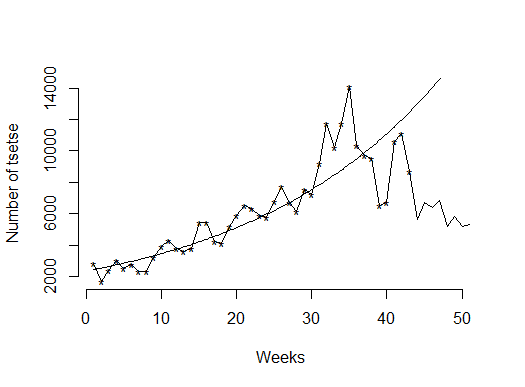
\includegraphics[width=0.9\linewidth]{Feb_06_fitGrouwthRate}
	\caption{The vertical axis is the estimated \textit{G. m. morsitans} female population on Antelope Island, Lake Kariba, Zimbabwe, from January 14th to December 30th, 1981. The time is measured in weeks, the blue line shows the model fit, and the red dots are the population estimates used in the fitting procedure.}
	\label{fig:antelopeEst}
\end{figure}


\newpage
We fitted an exponential function to the population estimates using the function \textit{fit\_easylinear()} from the R package "growthrate" (Figure \ref{fig:antelopeEst}). The weekly growth rate $r_m$ from the model fit is 0.03879 per week (sd: 0.002631 and $R^2$ = 0.837). We then used the $r_t$ estimate to calculate the weekly growth rate as a function of the weekly average temperatures from January 14th to December 30th, 1981, and then calculated $\hat{r}$, the long-time average value of $r_t$ for the year, by summing the weekly growth rate during this period and dividing by the total number of weeks (Equation \ref{equation1010}). The average growth rate during this period is 0.03851 per-week, with standard deviation 0.01461. The two estimates, arrived at by two entirely independent methods, using quite different approaches, thus gave very similar estimates – indicating that the $E-L$ method provides a reasonable way of estimating mean  growth rates over extended periods.


\subsection*{Sensitivity Analysis}
In a recent study \cite{are2019weakest}, an extensive sensitivity and uncertainty analysis was done on the extinction probabilities for populations of tsetse. The study derived an expression for the extinction probabilities for the flies' population and assessed the impact of each input parameter on the extinction probability. Here, in  a similar fashion to \cite{are2019weakest}, we aim to determine the parameters that have the strongest impact on the magnitude of the intrinsic rate of natural increase $r$. Hence, we define probabilities $p_l$, $p_c$ and $p_o$ respectively as: $p_l=e^{-\Psi \tau} $, $p_o =\epsilon e^{-\Omega \nu}$ , and $p_c =\beta e^{-\chi g}$.  Where: 
\begin{itemize}
	\item $\beta$ : Probability a deposited larva is female
	\item $\chi$ : Pupal daily mortality
	\item $\epsilon$: Probability of fertile insemination
	\item $g$: Pupal duration
	\item $\nu$: Time from emergence to first ovulation 
	\item $\Omega$: Daily mortality in immature adults 
	\item $\Psi$ : Daily mortality in larvipositing adults 
	\item $\tau$: Inter-larval period
\end{itemize}
For the sensitivity analysis, we assume that the number of male tsetse  in the population is always sufficient, such that all virgin females in the population are inseminated around the eighth  day of their emergence as adults $(\epsilon = 1)$. 
\paragraph{}
We use the Latin Hypercube Sampling (LHS) method and obtain the Partial Rank Correlation Coefficient (PRCC) for the intrinsic growth rate with respect to all input parameters (See \cite{are2019weakest} for details on the methodology).  Sensitivity analysis shows that the intrinsic rate $r$ is most sensitive to daily mortality $\Psi$ in larvipositing adults, followed by daily mortality $\chi$ in female pupae, and daily mortality $\Omega$ in immature adults. As expected, these three parameters, together with the inter-larval period $\tau$ and pupal duration $g$, all have negative impact on $r$ (Fig \ref{fig:SensitivityPlot}). This again reinforces the conclusion reached in \cite{are2019weakest} that increasing daily adult mortality for female tsetse is the most effective way of controlling/eradicating populations of tsetse.   



\begin{figure}[hbt!]
	\centering
	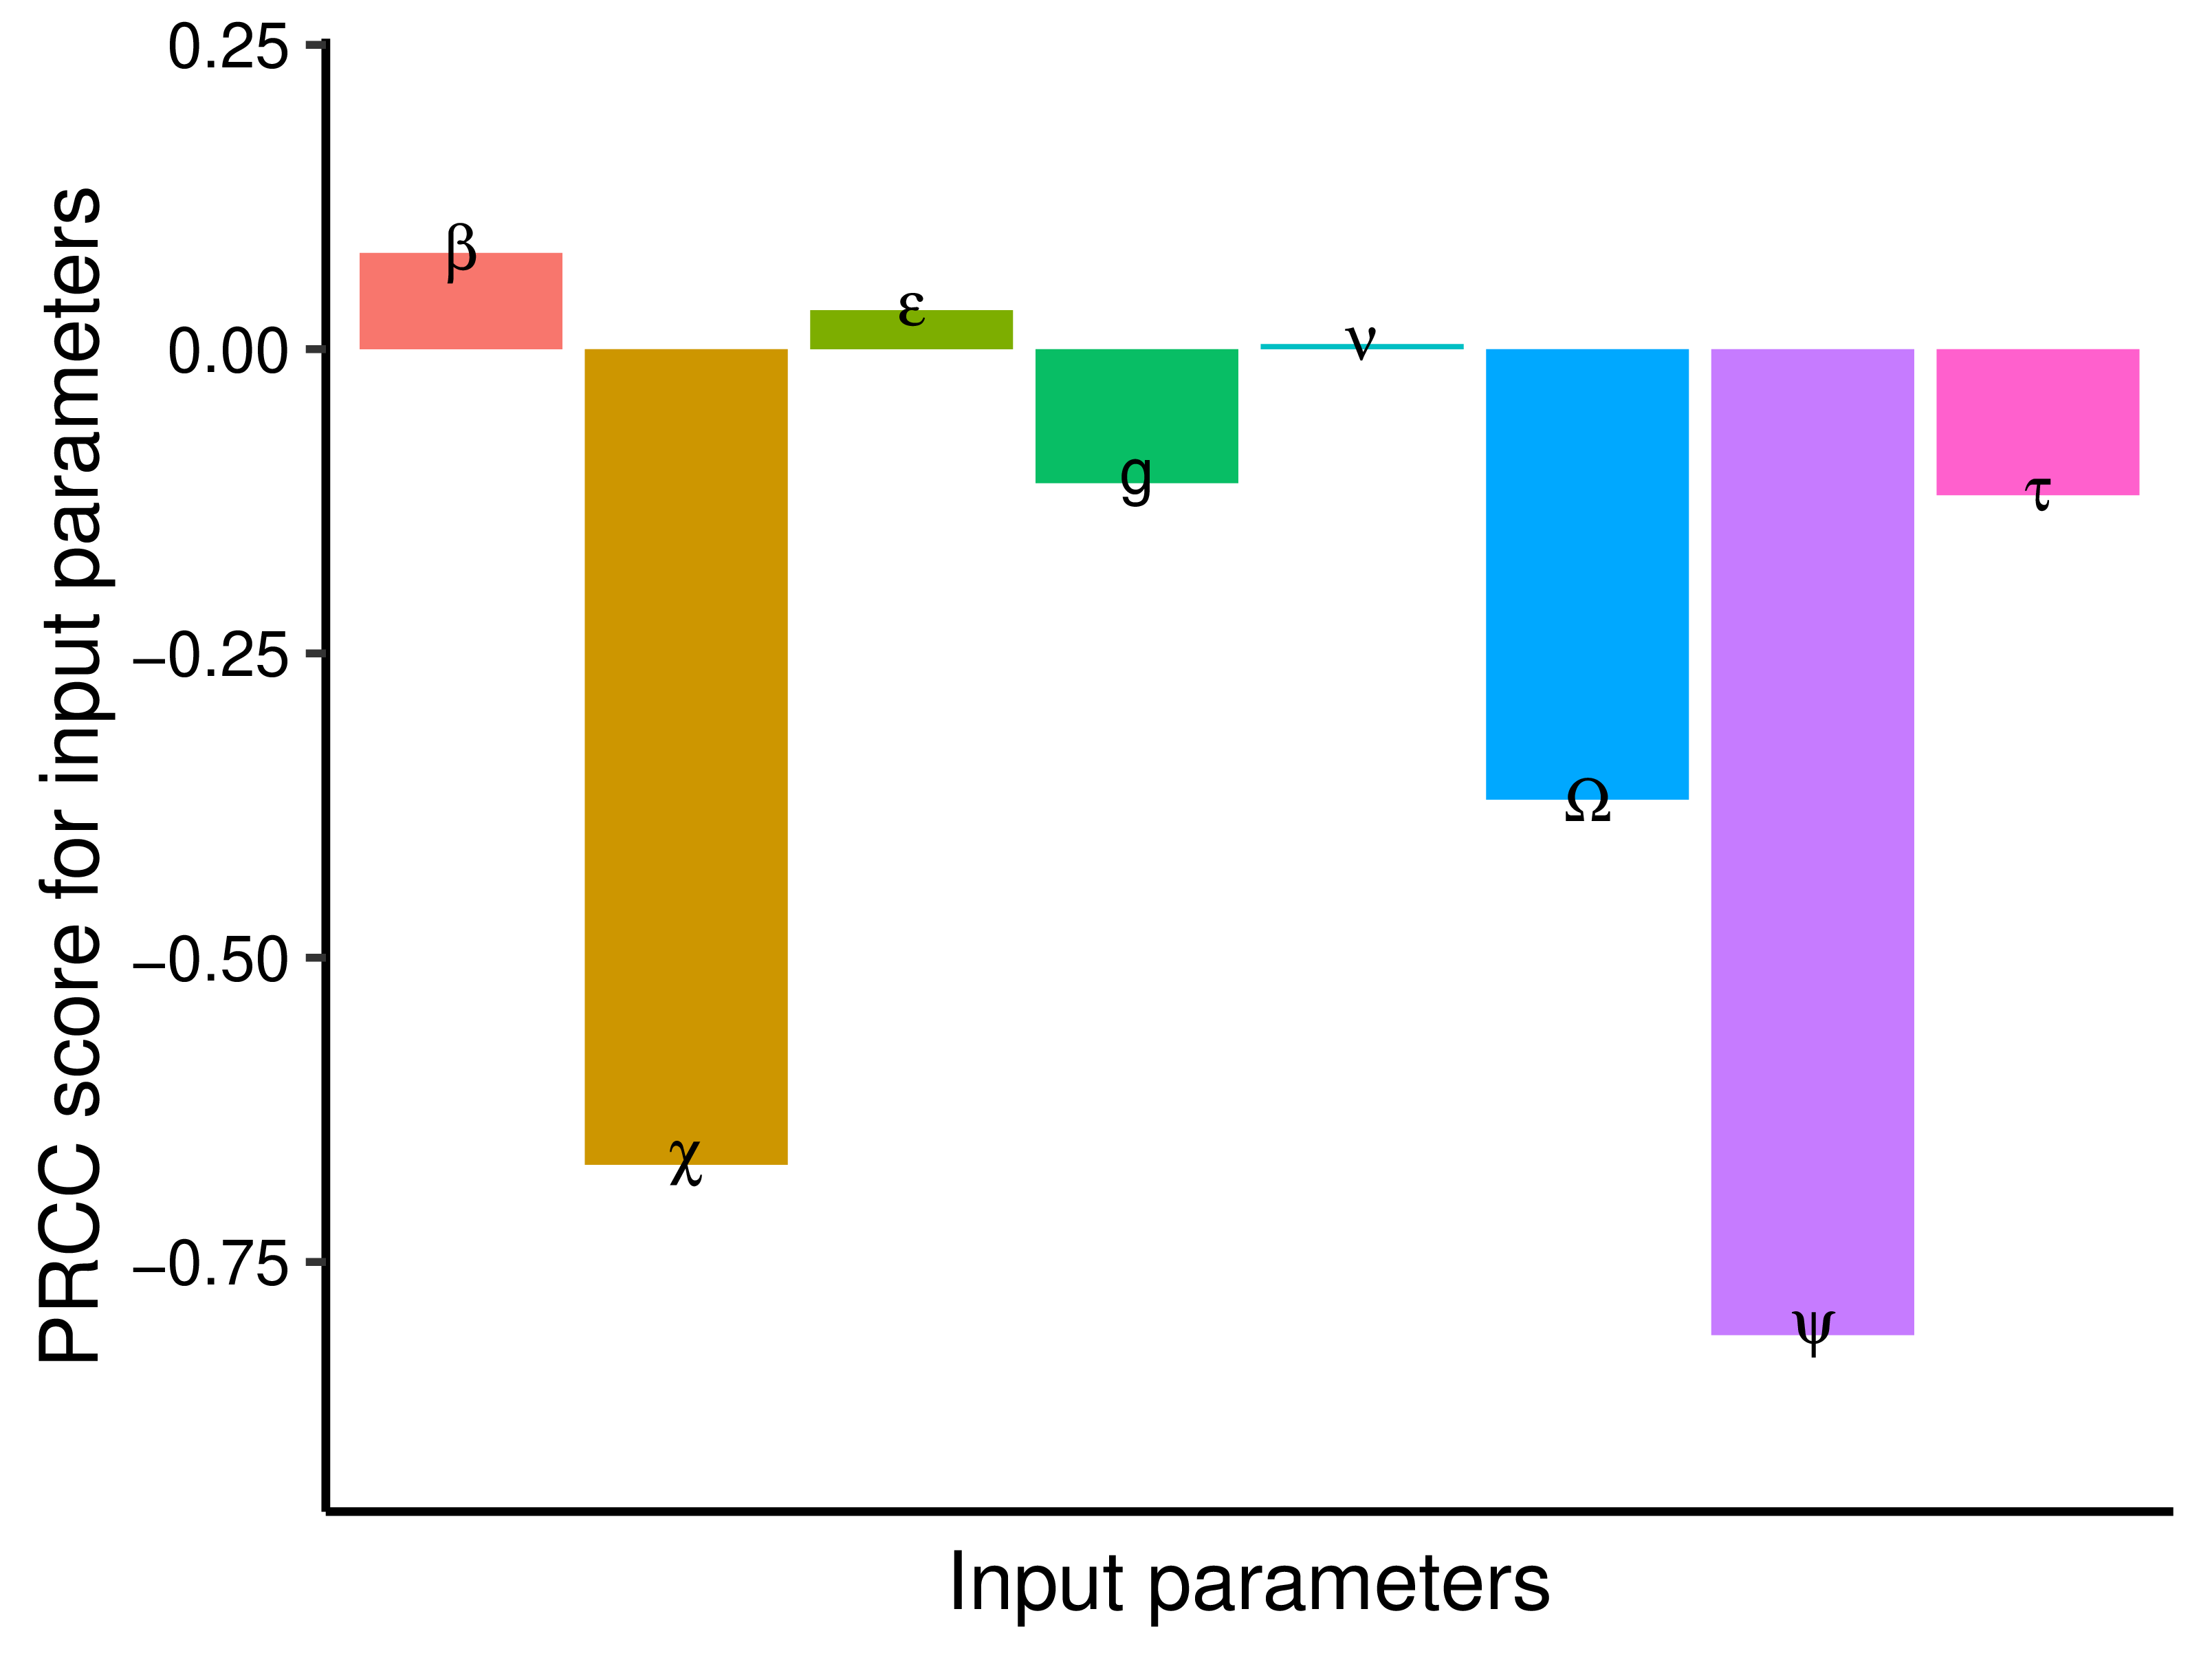
\includegraphics[width=0.7\linewidth]{GrowthRateSensitivityPlot}
	\caption{{\bf PRCC score for all eight model input parameters}. $\beta$: probability a deposited larva is female, $\chi$: pupal daily mortality, $\epsilon$: probability of fertile insemination, $g$: pupal duration, $\nu$: time from emergence to first ovulation, $\Omega$: Daily mortality in immature adults, $\Psi$: daily mortality in larvipositing adults, and $\tau$: inter-larval period.}
	\label{fig:SensitivityPlot}
\end{figure}

\subsection*{Temperature Data}
Between November 1959 and December 2018, daily maximum and minimum temperatures have been recorded at Rekomitjie using a mercury thermometer placed in a Stevenson screen.  Mean temperatures over 24-hour, and longer periods were approximated using the average of the daily maximum and minimum temperatures. We present the annual mean temperature at Rekomitjie, from 1960 - 2018 (Fig \ref{fig:AnnualAveTem}). Annual mean temperature  fluctuate quite widely between years at Rekomitjie, but have remained consistently above 25 \degree C since 1987. It is clear that Rekomitjie is getting hotter, and the rate at which the annual average temperatures depart from the optimal temperature for tsetse population growth (25 \degree C) \cite{Are2019} has continued to increase.  

\begin{figure}[hbt!]
	\centering
	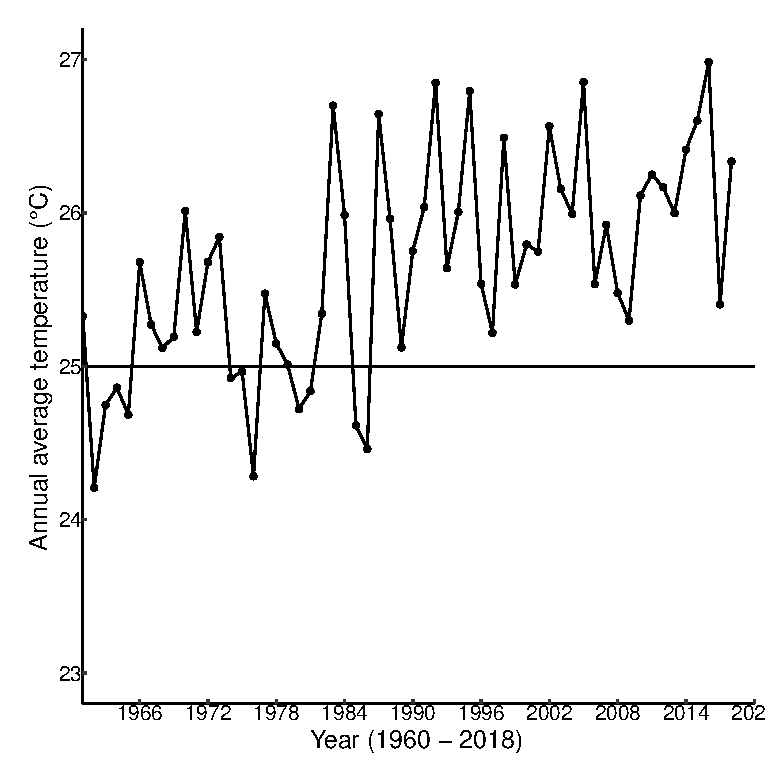
\includegraphics[width=0.7\linewidth]{20April20AnnualAverageTemp1960to2018}
	\caption{{\bf Annual mean temperature for Rekomitjie Research Station (1960 - 2018) .} The line through 25\degree C indicates the optimal temperature for tsetse population survival and reproduction.}
	\label{fig:AnnualAveTem}
\end{figure}


\newpage
We assess the differential changes in temperature between seasons for the study period. During the hot-wet season (January-April), the variation in monthly mean temperature has been minimal when compared to the fluctuation in the monthly mean temperature during the hot-dry season (September - December) where extreme temperature events have increased, both in intensity and in frequency  (Fig\ref{fig:combineTem} A \& C). Further details about the temperature data are provided elsewhere \cite{Lord2018}.     


\begin{figure}[hbt!]
	\centering
	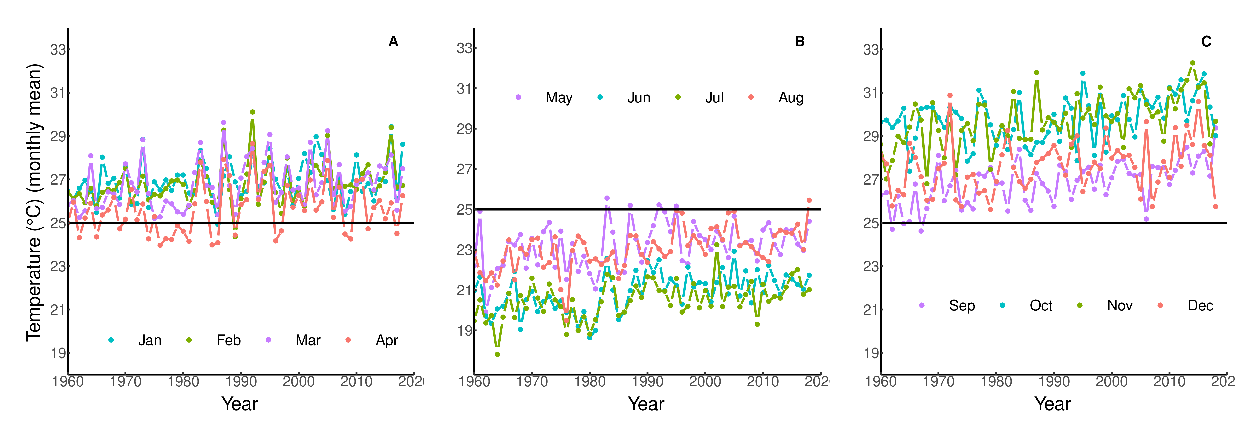
\includegraphics[width=1.1\linewidth]{21April20CombineTemPlot}
	\caption{{\bf Monthly mean temperature in Rekomitjie for different seasons (1960 - 2018) }. Monthly average temperatures for months in A. the hot-wet season (January - April)  B.cool-dry (May-August) and C. hot-dry (September-December). The line through 25\degree C indicates the optimal temperature for tsetse population survival and reproduction}
	\label{fig:combineTem}
\end{figure}


\newpage
\subsection*{Changes in age distributions with month of the year in Rekomitjie}
High temperatures in Rekomitjie have serious implications for tsetse population dynamics. For instance, studies have suggested that tsetse population age structure will be altered during the hot-dry seasons in Rekomitjie due to high temperature-induced mortality in pupae and newly emerged adults \cite{Hargrove2013b,hargrove2015mortality,Ackley2017}. An earlier study \cite{VanSickle1988} suggested that tsetse population will seldom, if ever, achieve a stable age distribution in Rekomitjie because once disproportionate mortalities affect pupae and young adults during the hot-dry season, the age distribution will not stabilise before the next hot-dry season sets in. In this study, we investigate this matter further by analysing the data collected on the ovarian age distribution for \textit{G. pallidipes} caught in traps at Rekomitjie from September 1988 – December 1999. We calculate chi-squared statistic for tsetse age distribution for consecutive months throughout the study period. A small chi-squared statistic will indicate similar age distribution structure between two consecutive months, while a large chi-squared statistic will imply a shift in the age distribution.  Our results show that the chi-squared statistic   is relatively small for the difference in ovarian age distribution from February to August. However, from September to January the chi-squared statistic increases rapidly, indicating a large shift in the age distribution during the hot-dry season (Fig \ref{fig:ChiSqrSttistic})

\begin{figure}[hbt!]
	\centering
	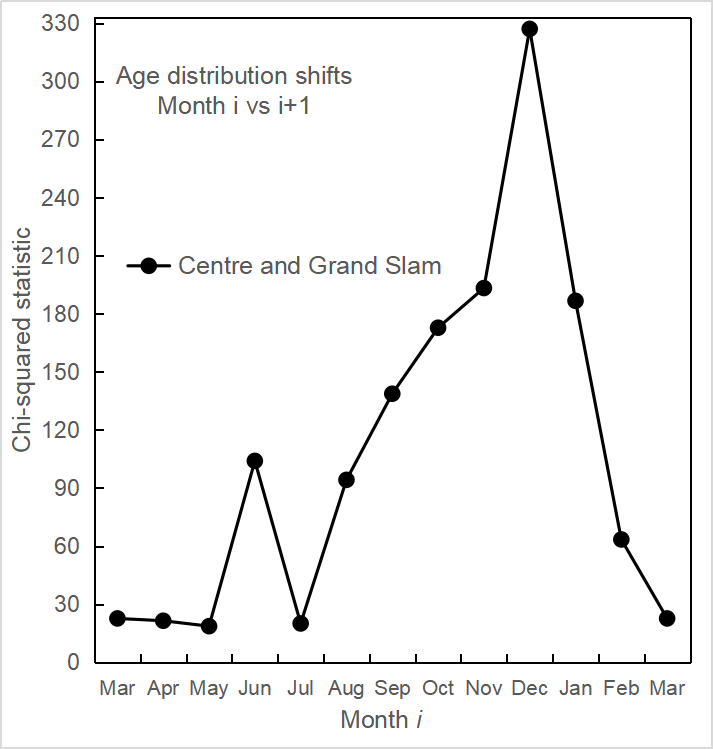
\includegraphics[width=0.7\linewidth]{ChiSqrSttistic}
	\caption{{\bf Chi-squared statistic for the difference between ovarian age distributions of tsetse caught in month $i$ vs month $i+1$.} \textit{G. pallidipes} captured in traps at Rekomitjie Research Station, September 1988 – December 1999. Total sample size 96,111. }
	\label{fig:ChiSqrSttistic}
\end{figure}

We compare the difference between age distribution for the two consecutive months with the smallest (May - June), and largest (December - January) chi-squared statistic, respectively. Essentially the age distributions in June and July have the same shape, whereas in December, the shape of the age distribution differs clearly from that of January. 
\begin{figure}[hbt!]
	\centering
	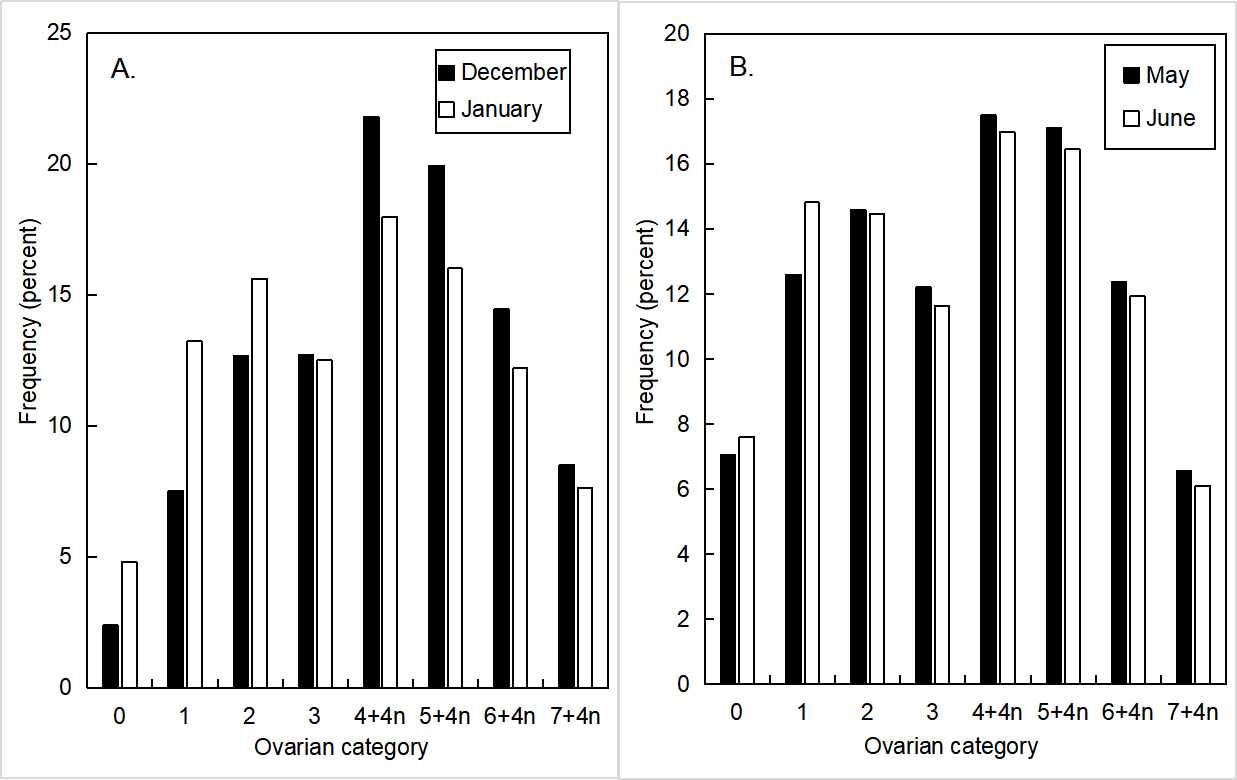
\includegraphics[width=0.9\linewidth]{AgeDistJUNJULDECJAN}
	\caption{{\bf Ovarian age distributions for \textit{G. pallidipes} caught in traps at Rekomitjie Research Station, September 1988 – December 1999}.  Graphs show results for months where there was the biggest (A) or smallest (B) change in percentage age distribution between months. Samples sizes: December 8711; January 8887; May 9634; June 5574. }
	\label{fig:AgeDistJUNJULDECJAN}
\end{figure}




\newpage
\subsection*{Climate change scenarios}

Over the past 27 years at Rekomitjie, average daily temperatures have increased by 2\textdegree C in the month of November, and by 0.9\textdegree C for the rest of the year \cite{Lord2018}.  Here we investigate the impact on the annual growth rates of tsetse population assuming that average temperatures continue to increase over the next 50 years at rates of either 0.04, 0.06 or 0.08 \textdegree C per-year. We are particularly interested to know what level of temperature increase would cause tsetse population growth rates to become consistently negative.

\section*{Results}
We used the daily average temperature data and equation (\ref{equation13}) to predict the intrinsic rate of natural increase of tsetse population in the neighbourhood of Rekomitjie, for each day between January 1960 and December 2018. We then used equation (\ref{equation1010}) to obtain annual averages for $r$. Notice that all references below to growth rates are values predicted from temperature profiles.   
\paragraph{}
From 1960 to 1986, the annual average growth rate was relatively stable, varying between 0.0031 and 0.00389.  Between 1987 and 1995, however, the growth rate dropped below the previous minimum of 0.0031 in four of the nine years, with a low of 0.00287 in 1992, during which year catches of tsetse at Rekomitjie also fell to their lowest recorded levels up to that time \cite{hargrove2015mortality}. There followed a slow recovery with increased growth rates until 2009. Thereafter, rates fell consistently, hitting an all-time low of 0.0023 in 2016 (Fig \ref{fig:tsetseflowchat0}), at which time catches were also at an all-time low \cite{Lord2018}.


\begin{figure}[hbt!]
	\centering
	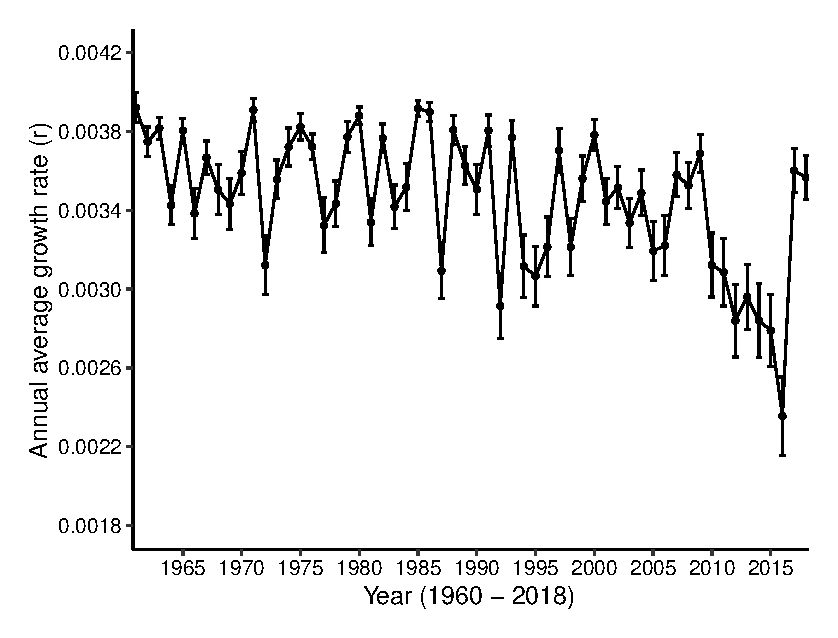
\includegraphics[width=0.8\linewidth]{GratewithErrBars}
	\caption{Averaged annual growth rate for tsetse population at Rekomitjie Research Station, Zambezi Valley, Zimbabwe: from 1960 to 2018.}
	\label{fig:tsetseflowchat0}
\end{figure} 
Temperatures vary seasonally, and the highest temperatures at Rekomitjie are usually recorded at the end of the dry season in September – December. We classified the year into three seasons: hot-wet (January-April), cool-dry (May-August) and hot-dry (September-December). For each of these seasons we obtained the average growth for each month, separately, throughout the study period. This allowed us to assess the differential values of the average growth rate during the hot-dry months and the cooler seasons of the year. The average growth rate for January-April changed little over the years around an average value of 0.004, save for 1996 and 2016 when the average growth rate dropped markedly in January and February (Fig \ref{fig:tsetseflowchat2}A).  
\paragraph{}
For March-April, the average growth rate varied even less. The growth rate attains it highest value, during this period, the growth rate is about 0.0045. The average growth rate was consistently lower during June and July, the coolest months of the year, than in May and August (Fig \ref{fig:tsetseflowchat2}B).  

\begin{figure}[h]
	\centering
	
\includegraphics[width=1.1\linewidth]{MonthlyGrowthRateDec12}
	\caption{ {\bf The average growth rate for different seasons from 1960 to 2018} (A). Average growth rate for January, February, March and April (B). Average growth rate for May, June, July and August (C). Average growth rate for September, October, November and December. The horizontal lines show the limit of positive growth; below those lines the population size decreases}
	\label{fig:tsetseflowchat2}
\end{figure}

\newpage

By far the greatest variation in the average growth rate, both within and between years, occurs during the last four months of the year, particularly in October and November. Between 1987 and 2018, the average growth rate has been negative for 22  out of 32 years, during these two months. In 2014, the growth rate dipped below -0.005 - the lowest monthly average ever (Fig \ref{fig:tsetseflowchat2}C). Variation in average growth rates for September were much less pronounced than for the other three months of the hot-dry season. From 2010 to 2018, there has been increased variation in the growth rate during the last three months of the year. 


\begin{figure}[h]
	\centering
	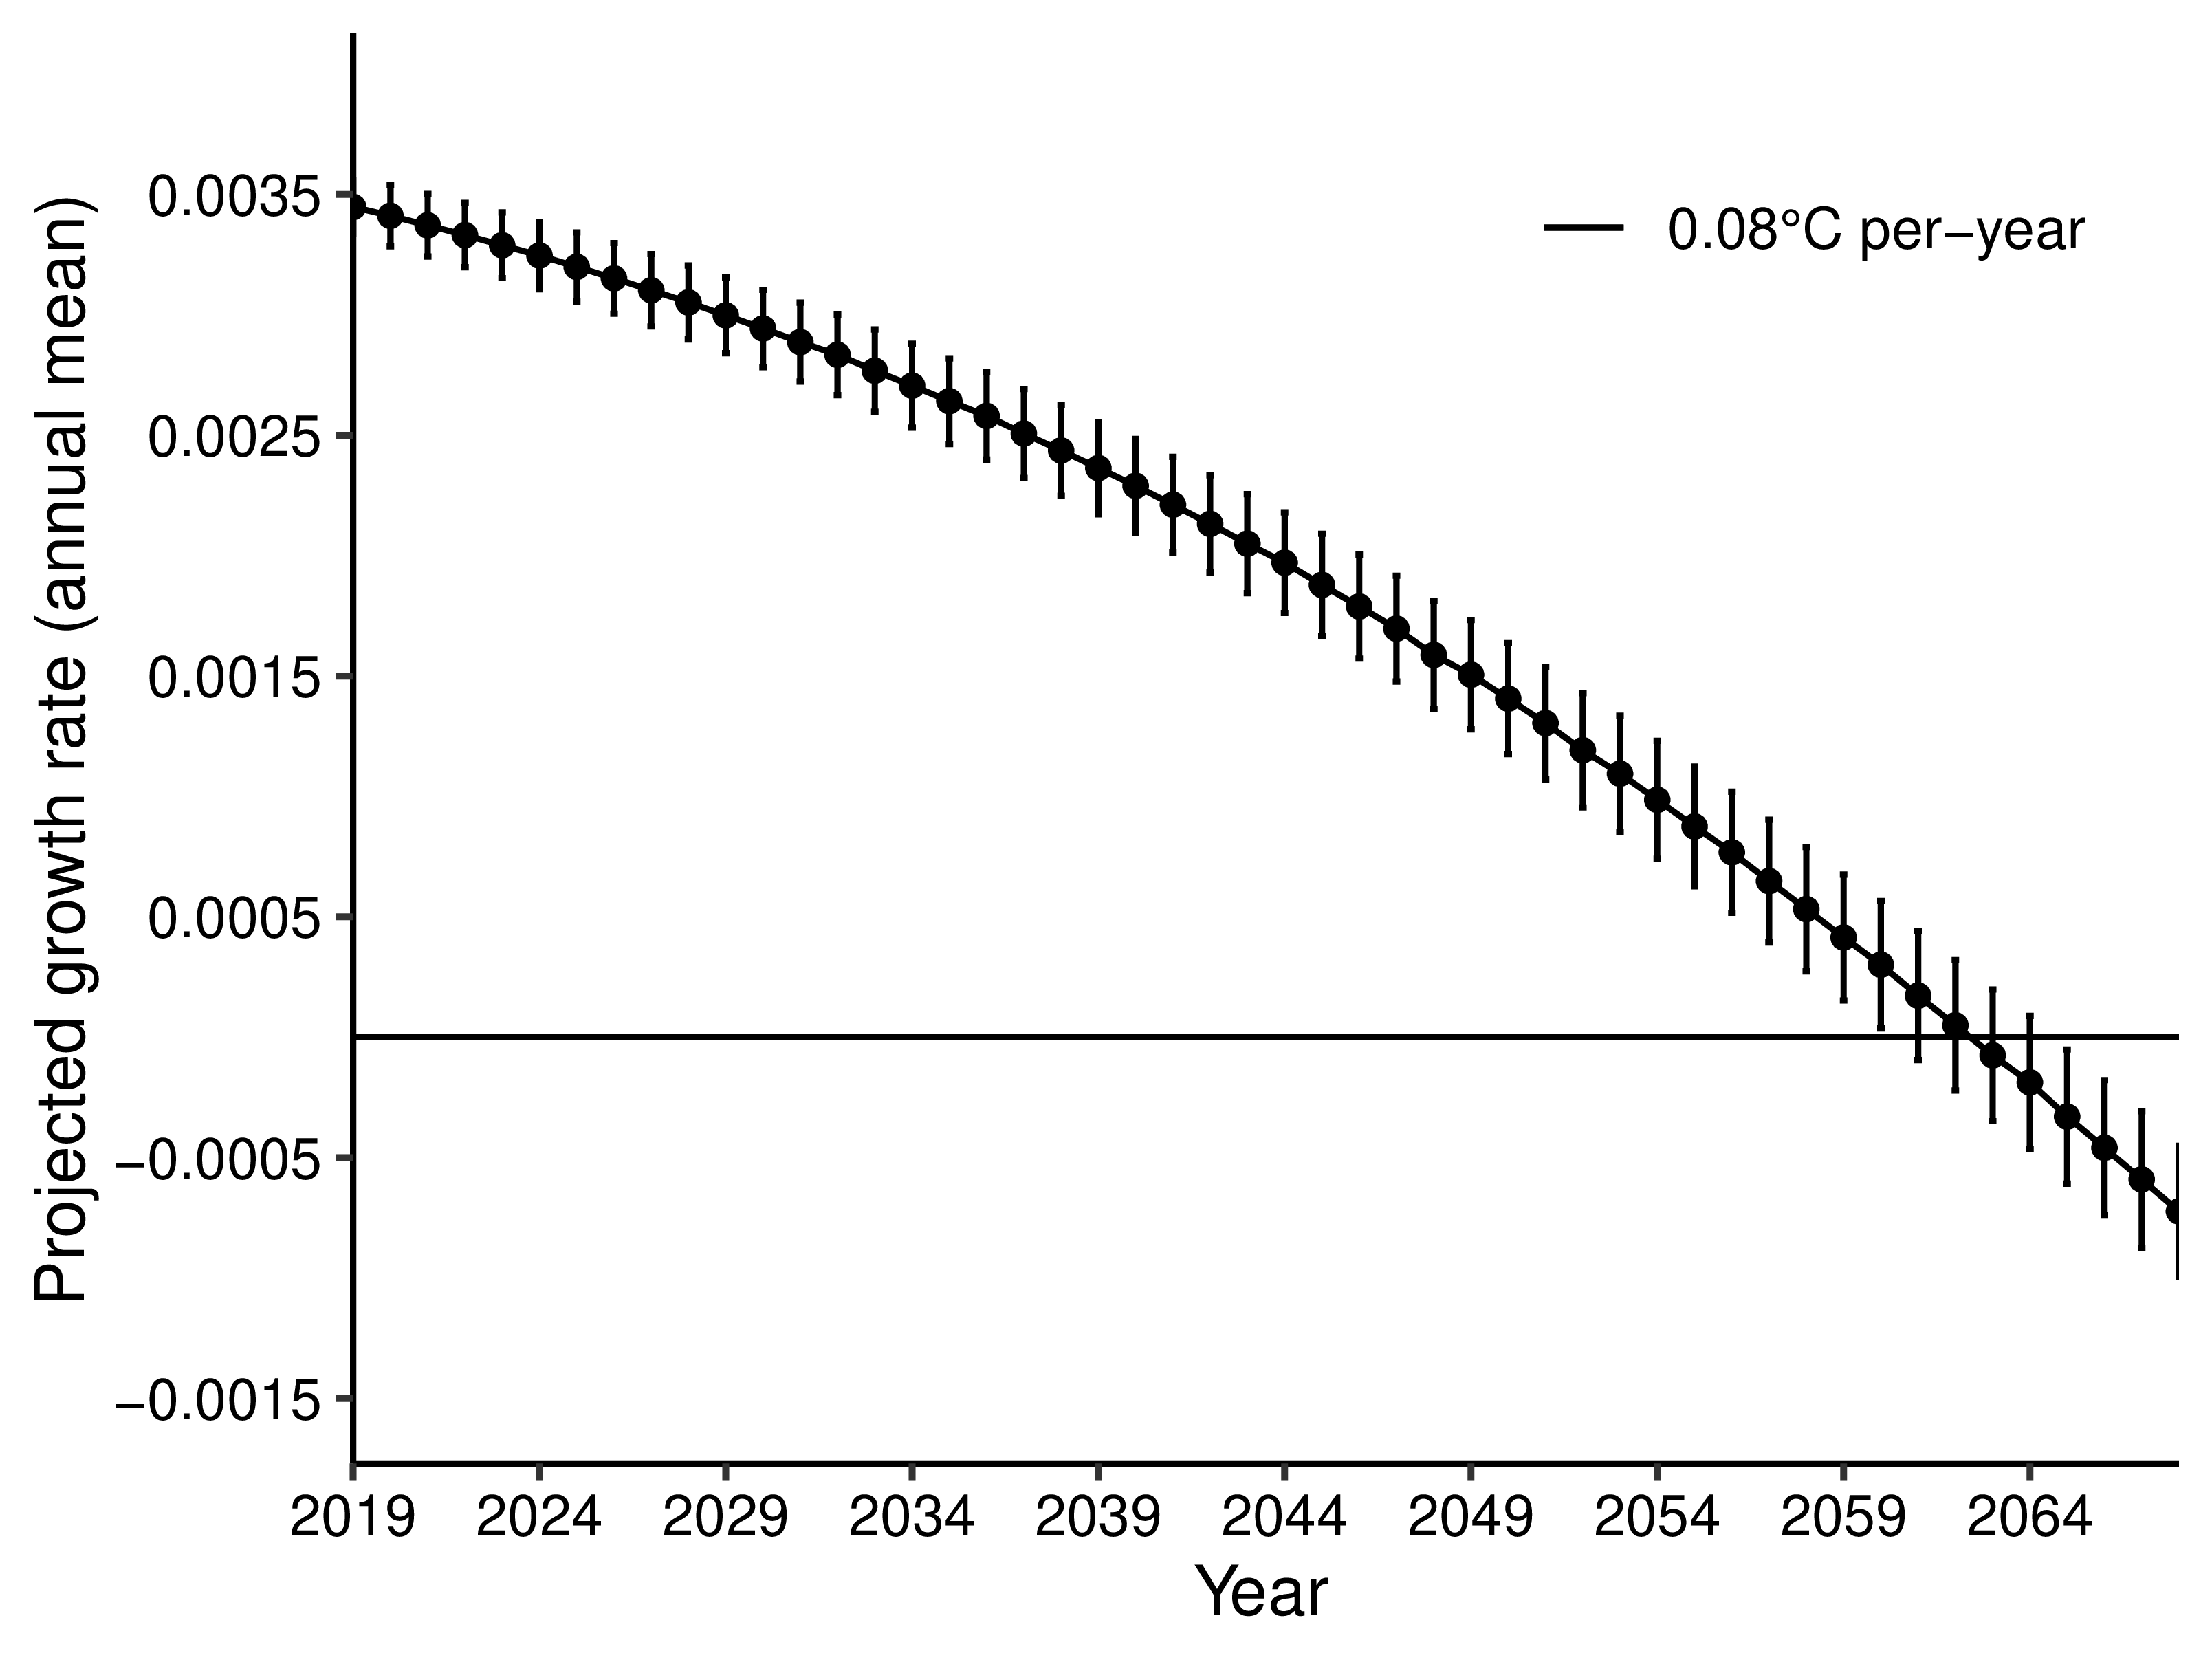
\includegraphics[width=0.8\linewidth]{ProjectionwithErrBar}
\caption{{\bf The annual average growth rate for the three projected climate change scenarios (0.04, 0.06, 0.08 \degree C per-year), from 2019 to 2068}. The horizontal line, through the vertical axis, shows the point where the average growth rate attains negative values: indicating population extinction. Extinction did not occur within the next 50 years for 0.04 and 0.06 warming rates}
	\label{fig:tsetseflowchat4}
\end{figure}

\subsection*{Projected growth rates at Rekomitjie assuming different rates of temperature increase}
We created three climate change scenarios over the next 50 years, using 2018's daily average temperature as the baseline. We used these temperature projections to calculate the annual average value of the growth rate from 2019-2068.
\paragraph{}
When the warming rate is slow (at 0.04 \textdegree C per-year), the average growth rate continues to decline as temperature increases, but does not reach a negative value within the next 50 years. For the scenario where the warming rate is 0.06 \textdegree C per-year, the $\hat{r}$ drops below 0.001 but did not reach a negative value. It is only when the warming rate is increased to 0.08 \textdegree C per-year that $\hat{r}$ declines steadily until it reaches a negative value in 2063. If negative $\hat{r}$ values are sustained the population will eventually become extinct.

 
\section*{Discussion}
It has been suggested that temperature increases at Rekomitjie led to a collapse in tsetse population in that region after 2010 \cite{Lord2018}. The study suggested that, if temperatures continue to increase, there could be local extinctions of tsetse population in the Zambezi valley.  The current study used temperature data from Rekomitjie to estimate how tsetse growth rates have changed in the neighbourhood of the Station over the past 60 years. It also predicted the changes that will occur in future growth rates, given different climate change scenarios.  We solved the E-L equation analytically, and we obtained a closed form expression for the intrinsic growth rate $r$ for tsetse populations. To validate our model results we used weekly average temperature readings for Antelope Island, Lake Kariba, Zimbabwe, in 1981, to estimate the average growth rate for 1981 for a population of \textit{G. m. morsitans} on the island. We compared our results to the growth rate obtained by fitting an exponential function to weekly estimates of female tsetse population, over the same period (1981). Our model results compare well with the estimates from the exponential model fitted to the mark-recapture population estimates. This is expected because the tsetse population on the island in 1981 was growing from a low base and numbers were much lower than the carrying capacity. We expect, therefore that density dependent effects would not have been important. In this case, the actual population growth rate should be very close to the intrinsic rate of increase.
\paragraph{}
We used daily average temperatures recorded at Rekomitjie, from January 1960 to December 2018, to calculate the long-time average values of $r$. Using the temperature readings for 2018 as a baseline, we projected three climate change scenarios, by projecting daily average temperatures for Rekomitjie over the next 50 years, following three climate warming rates. We used the projected temperatures to calculate the long-time averages of the growth rate. 
\paragraph{}
Our results show that annual population intrinsic growth rates for tsetse at Rekomitjie have fluctuated quite widely between years over the past 60 years, but there was no strong trend in the rates between 1960 and about 2009. Thereafter, however, average temperatures have increased markedly, and annual average growth rate have declined, most sharply since 2010.  Our results agree with several studies \cite{Pagabeleguem2016f,Ackley2017}, both empirical and theoretical, that have shown that high temperatures are devastating for tsetse populations, and that increasingly high temperatures can drive tsetse populations to extinction \cite{Lord2018,Are2019}. Our results offer insight into how very high temperatures during the hot-dry season are responsible for the decline in tsetse population at Rekomitjie. During the hot-dry seasons, high mortality rates in both pupal and newly emerged adult stages, due to high temperatures \cite{Ackley2017}, can explain the negative growth rates during these months.  As global warming continues to increase the average temperatures at Rekomitjie all year round, tsetse populations will not be able to recover fully from the disastrous impact of the hot-dry season before the next hot-dry season sets in. This may possibly explain the decline in tsetse population, at Rekomitjie, over the past 10 - 20 years. 
\paragraph{}
Our intrinsic growth rate estimates for Rekomitjie, on the other hand, may  be seen as the upper bound for the actual population growth because of the following reasons: (1) Our modelling framework did not consider density dependent effects. In practice, effects such as density dependent mortality will limit population growth when the population approaches its carrying capacity. At these times the actual growth rate for tsetse populations will not attain its intrinsic capacity. (2). For tsetse populations in the field, where temperatures vary seasonally, the very high temperatures during the hot-dry season destabilise the population age distribution through the particularly high losses experienced by pupae and newly emerge adults under these conditions  \cite{VanSickle1988,Hargrove2013b}, thereby preventing the actual growth rate from reaching its full potential. We can then expect the actual population growth rate to fall below our $r$ estimates. The foregoing two reasons may explain why, despite the observed decrease in tsetse populations at Rekomitjie, the annual average intrinsic growth rate, although reducing, is still positive as at 2018. The fact that the $r$ is reducing shows that Rekomitjie is becoming less suitable for tsetse populations to thrive. Moreover, our model projections suggests that  a warming rate of 0.08\textdegree C  will be sufficient to ensure that the intrinsic growth rate will become negative and it will be impossible for any tsetse population to survive at Rekomitjie beyond about 2063. 
\paragraph{}
We have shown that tsetse populations have very low growth rates. For instance, from the 1960s to 1980s where the environmental temperatures were relatively favourable throughout the year, the annual average growth rate was always below 0.004 per-year. This is consistent with the low birth rates found in tsetse \cite{Hargrove2004a,HARGROVE1988}. Other studies have also estimated very low population growth rates for tsetse populations \cite{VanSickle1988,Hargrove2004a}. We have assumed that no additional mortality is imposed on the study population either by control efforts or human activities e.g., bush clearing. If any of these assumptions are not true, tsetse growth rate will be lower than the values we predict here. Our result may therefore be a best-case scenario for tsetse populations which are experiencing the temperatures recorded at Rekomitjie during these periods. Our result can be seen as a maximum for the instantaneous growth rate attainable for tsetse populations at Rekomitjie. 
\paragraph{} 
% % % % % % % % % % % % % % % % % % % % % % % % % % % % % % %
% % % % % % % % %Age Distribution Discussion % % % % % % % % % 
We acknowledge that the E-L equation was premised on the assumption that the population attains a stable age distribution, and where the environment is not limited by resources or space. Our results agree in-part with findings from the previous studies on tsetse age distribution \cite{ VanSickle1988,Hargrove2013b,hargrove2015mortality,Ackley2017},  and also provides a clearer insight on what happens to tsetse age distribution within a year. We show that, although it is true that tsetse age distribution cannot be stable throughout each of the months in a year, however as soon as the hot-dry season passes, tsetse age distribution essentially stabilises from February of the preceding year up until August before the high temperatures again perturb the age structure significantly from September - January of the preceding   year. Moreover, Amarasekare et al \cite{Amarasekare2013} provided strong evidence that populations can still attain stationary age distributions as long as the fluctuation in environmental temperature is within a threshold that will allow reproduction and development processes to continue. We have shown that for most months of the year, at Rekomitjie, apart from the hot dry seasons, temperature variations have been minimal. The instability in the age distribution is often introduced during the hot-dry seasons \cite{Hargrove2013b} of the very hot years. Therefore, barring any density dependent effects, we would expect the actual growth rates to be close to the intrinsic rate of increase during seasons when population growth is optimal. Our estimates provide a very insightful first step towards more accurate estimates of tsetse population growth rate under varying temperatures.
% % % % % % % % % % % % % % % % % % % % % % % % % % % % % % % % % % % % % % %
\paragraph{} 
The current study did not consider density dependent effects, which are very important for tsetse populations \cite{Rogers1975}. However, the E-L equation has been shown to yield comparable estimates of $r$ to other methods that do incorporate density dependent effects \cite{Cortes2016}. Moreover, as tsetse populations continue to decline in Rekomitjie, due to high temperatures, density-dependent effects may fall off, since the population may lie far below its carrying capacity. . 

% A study \cite{Cortes2016} did an extensive comparison of five different methods for estimating $r$ for a fish population and they reported that the density independent assumption on which E-L equation is derived does not limit it validity of the $r$ estimates derived from it.        
\paragraph{} 
A study \cite{Amarasekare2013} compared the average growth rate calculated from the E-L equation to the one obtained from a stage-structured compartmental model. They reported that the growth rates obtained from the two methods were similar, deviating only when the juvenile developmental period is long (several months) and/or when projections involve long time-scales ($>$ 50 years).  When the two estimates differ, $r$ derived from the E-L equation overestimates the true growth rates, and by implication, it overestimates population persistence. They suggested that the accuracy of $r$, from the E-L method, declines if it is used to predict insect population extinction beyond a 50-year period.  The current study took these cautions into account. Moreover, tsetse developmental period can vary between 20 - 60 days depending on temperature, and it therefore can be categorized as having a relatively short developmental period. In any case, the shortcoming of our method will be that we may have slightly overestimated the intrinsic rate of increase, and therefore tsetse populations may more likely go extinct earlier than in 2063 as predicted by our results.
\section*{Conclusions}
The framework presented here is simple and relatively straightforward. We recognize that some of the shortcomings of our formulation may limit the accuracy of our estimates.  However, among other things, since we got a closed form expression for $r$, it will serve as a metric for easy comparison with future findings. Moreover, it is clear that this crude estimate provides strong evidence that climate change could drive tsetse populations to extinction within the next 50 years (with a medium warming rate of 0.08\textdegree C per-year), especially in regions with temperature profiles similar to those at Rekomitjie. If our results are true for other insects with similar reproduction/development processes to tsetse, then several insects, of agricultural and/or economic importance, may be at risk of extinction in the Zambezi Valley in particular, and Zimbabwe (or other part of Africa with similar temperature regimes as the Zimbabwe), in general. 
\paragraph{}
We are currently constructing an individual based model which will allow us to factor in several environmental variables at the same time, to estimate growth rate of tsetse populations in the wild. 




\bibliographystyle{ieeetr}
\nocite{*}
\bibliography{Growthrate}
\end{document}



%%%%%%%%%%%%%%%%%%%%%%%%%%%%%%%%%%%%%%%%%%%%%%%%%%%%%%%%%End of article%%%%%%%%%%%%%%%%%%%%%%%%%%%%%%%%%%%%%%%%%%%%%%%

